\chapter{Dark matter interpretations of Run 1 searches for invisibly decaying Higgs bosons}
\label{chap:interp}
As well as combining the results of the \ac{VBF} searches with other channels, it is also possible to interpret them as limits on other specific models. Interpretations of the \ac{VBF} search results in several \ac{DM} models are described in \SectionRef{sec:dminterp}.

%??CHECK PLOT AXIS LABEL SIZES AND THAT LEGEND TERMS ARE STANDARD OR IN TEXT

\section{Simulation Techniques and Validation}
\label{sec:dmval}

%??start with internal sample
%??validate against powheg plus delphes: when generated with same PU etc. found to agree to within 10%
%??validate powheg plus delphes against mg plus delphes table from phenoplots281015.pdf
\begin{table}
  \caption{}%??explain cuts added and turn into standard notation from here
  \label{tab:mgvspowhegdelphes}
  \begin{tabular}{lcc}
    \hline
    \hline
    Cut added & Madgraph + Delphes & Powheg + Delphes \\
    \hline
    Start point & 2653 & 2311 \\
    jet 1 $p_{T}>50$ GeV, jet 2 $p_{T}>45$ GeV & 2056 & 1834 \\
    MET$>90$ GeV & 2000 & 1793 \\
    $M_{jj}>1200$ GeV & 704 & 689 \\
    MET significance$>4$ & 539 & 519 \\
    min$\Delta\phi(j,MET)>2.3$ & 244 & 248 \\
    \hline
    \hline
  \end{tabular}
\end{table}

%??recreation of metsig and l1met
%??systematic scaling


\begin{figure}
  \subfloat[]{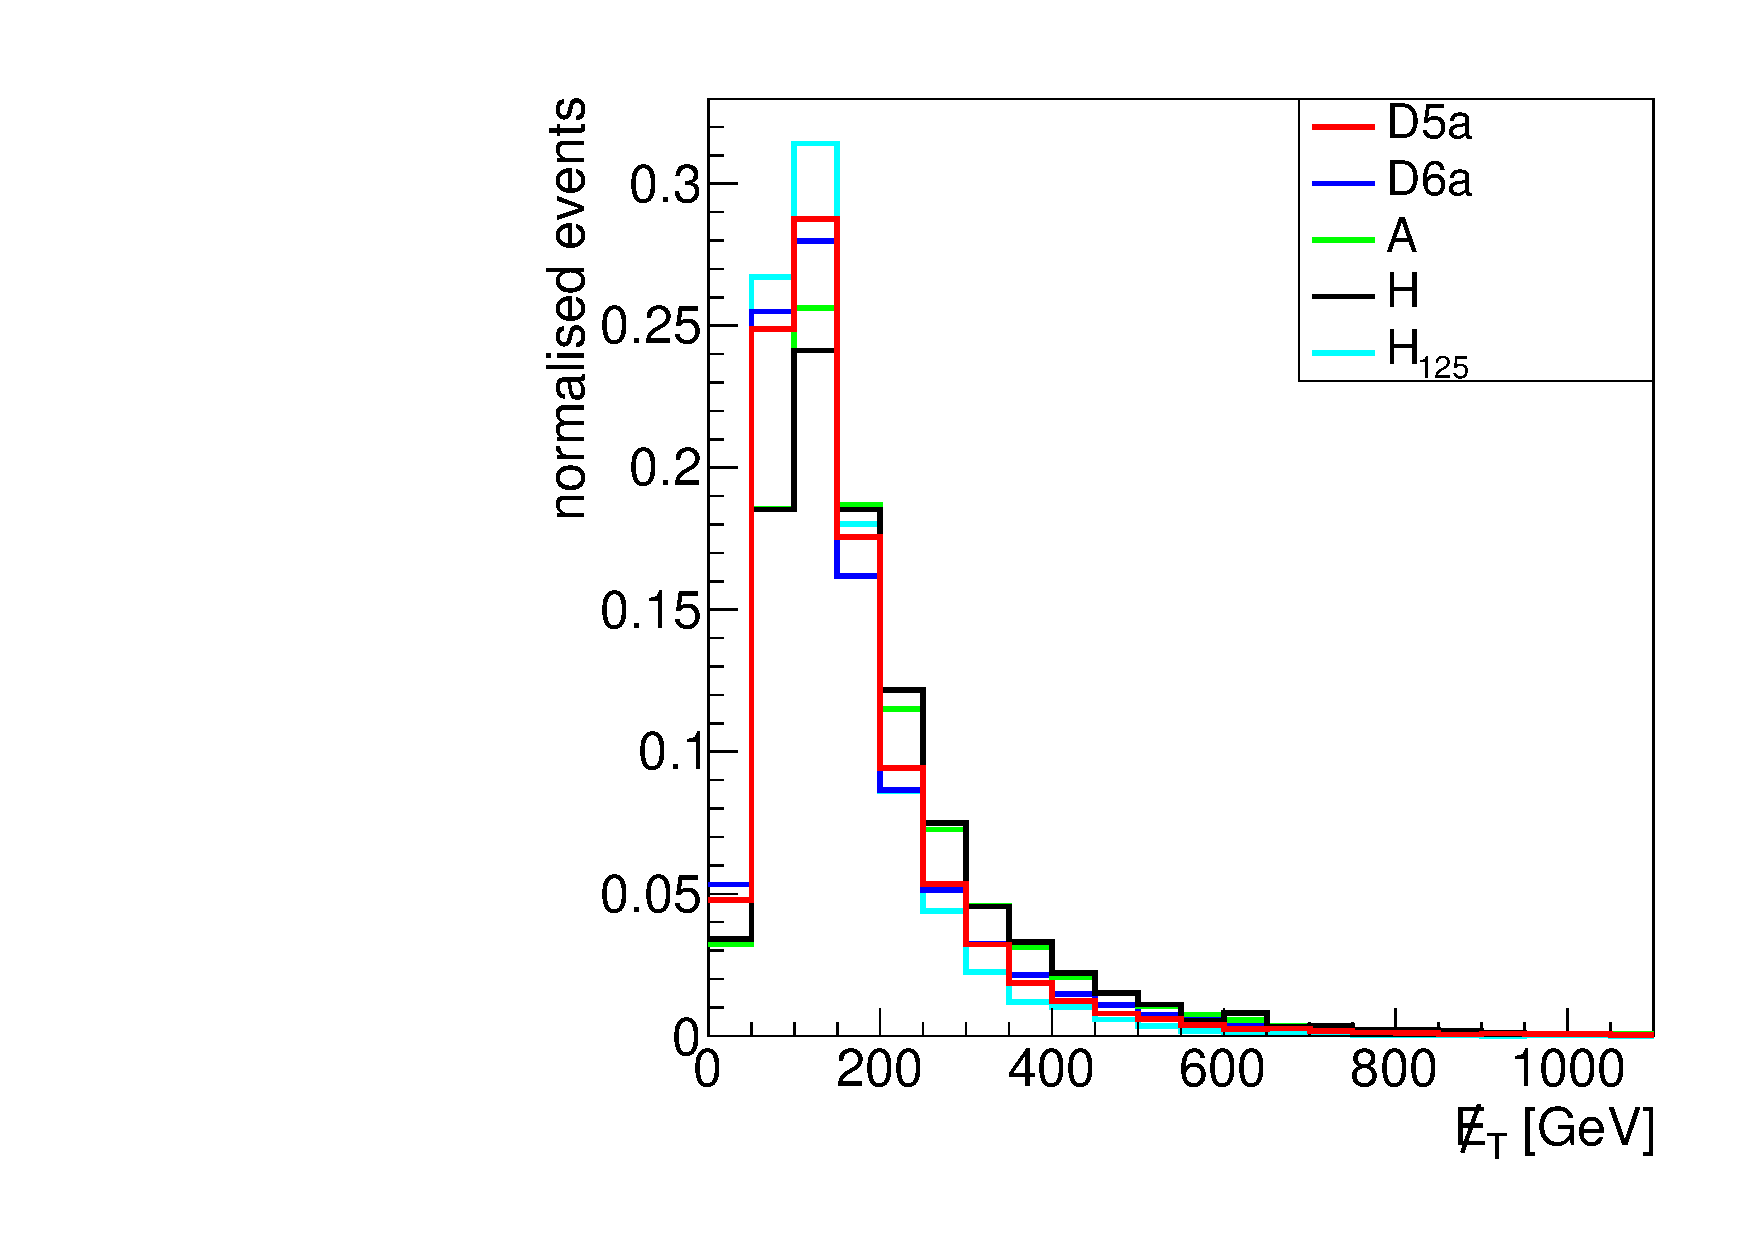
\includegraphics[width=.65\largefigwidth]{plots/interp/modelmet.pdf}}
  \subfloat[]{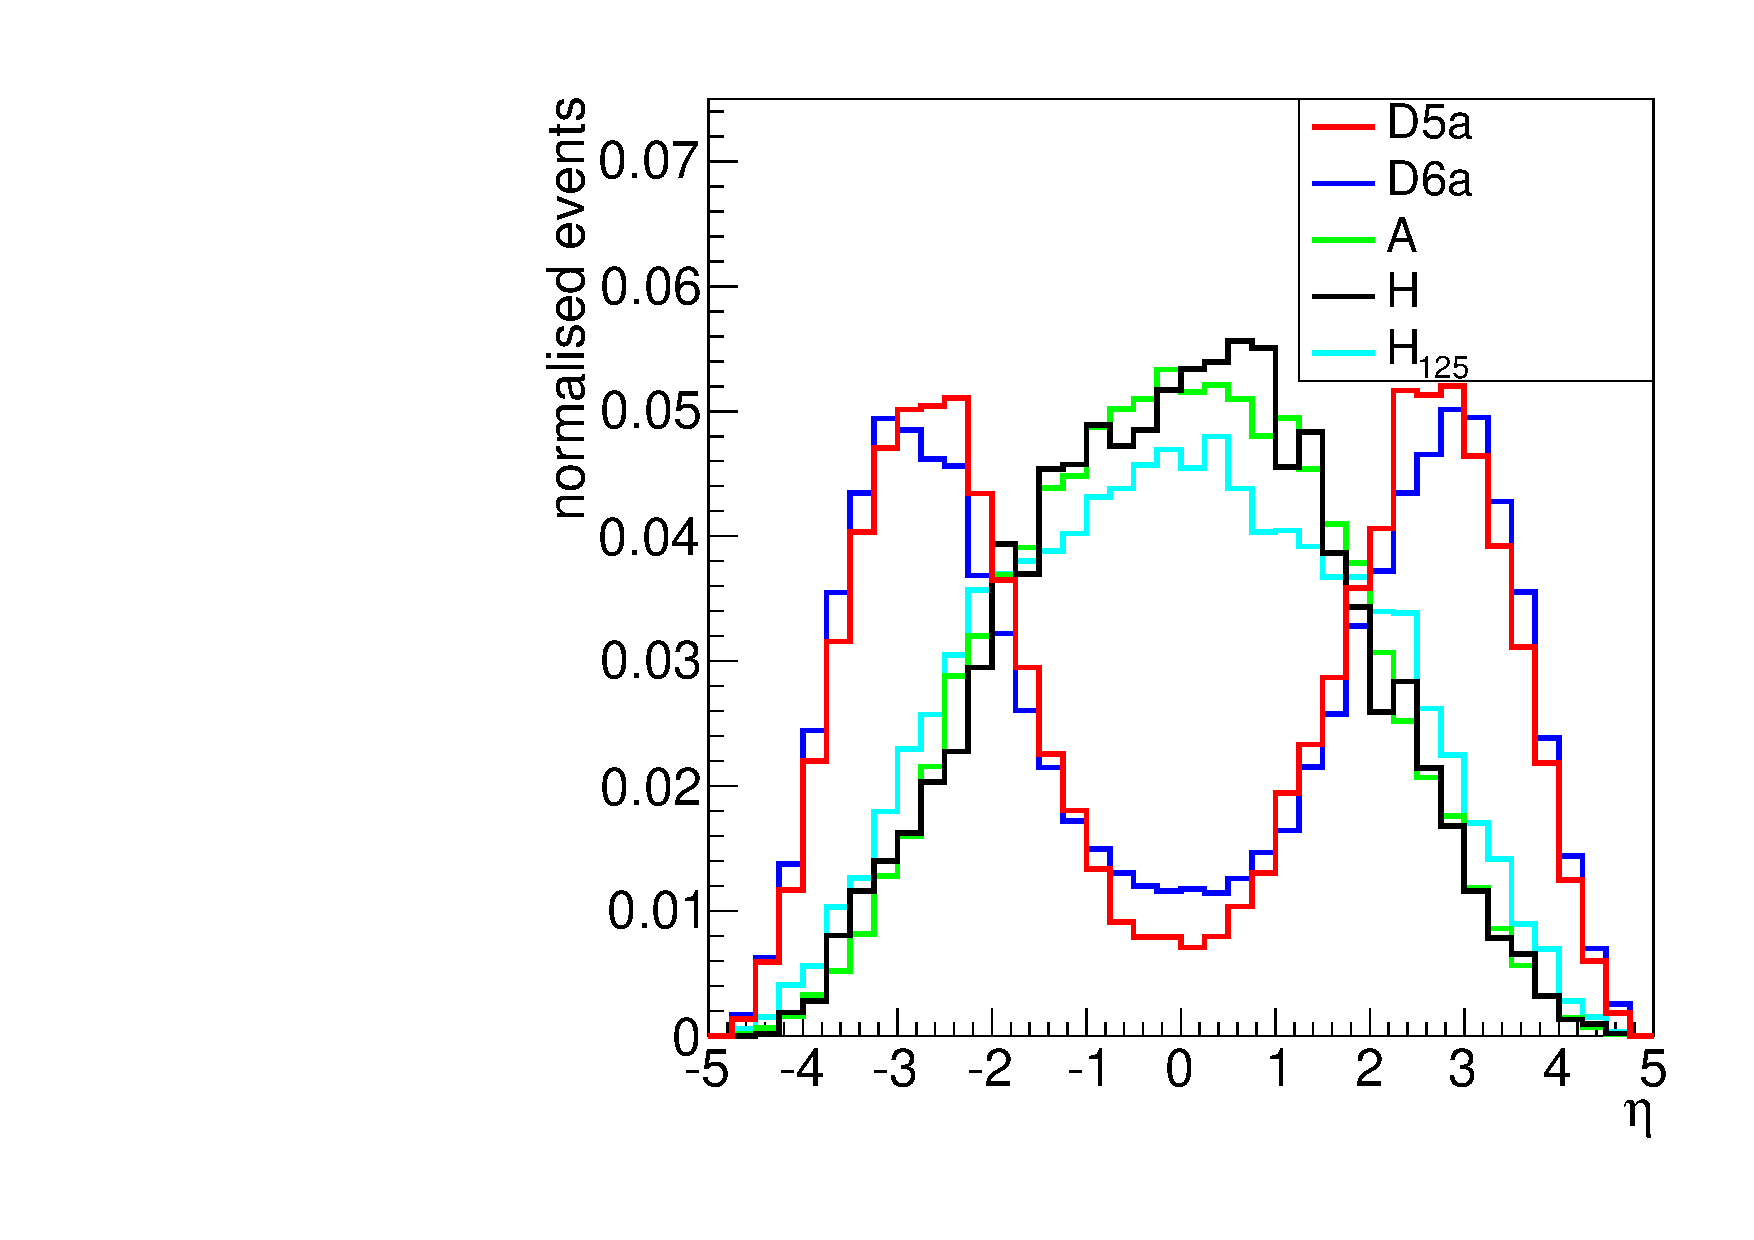
\includegraphics[width=.65\largefigwidth]{plots/interp/modeleta.pdf}}
  \caption{}%??
  \label{fig:dmmodelkinematics}
\end{figure}

\section{Results}
\label{sec:dmresults}

\begin{figure}
  \subfloat[]{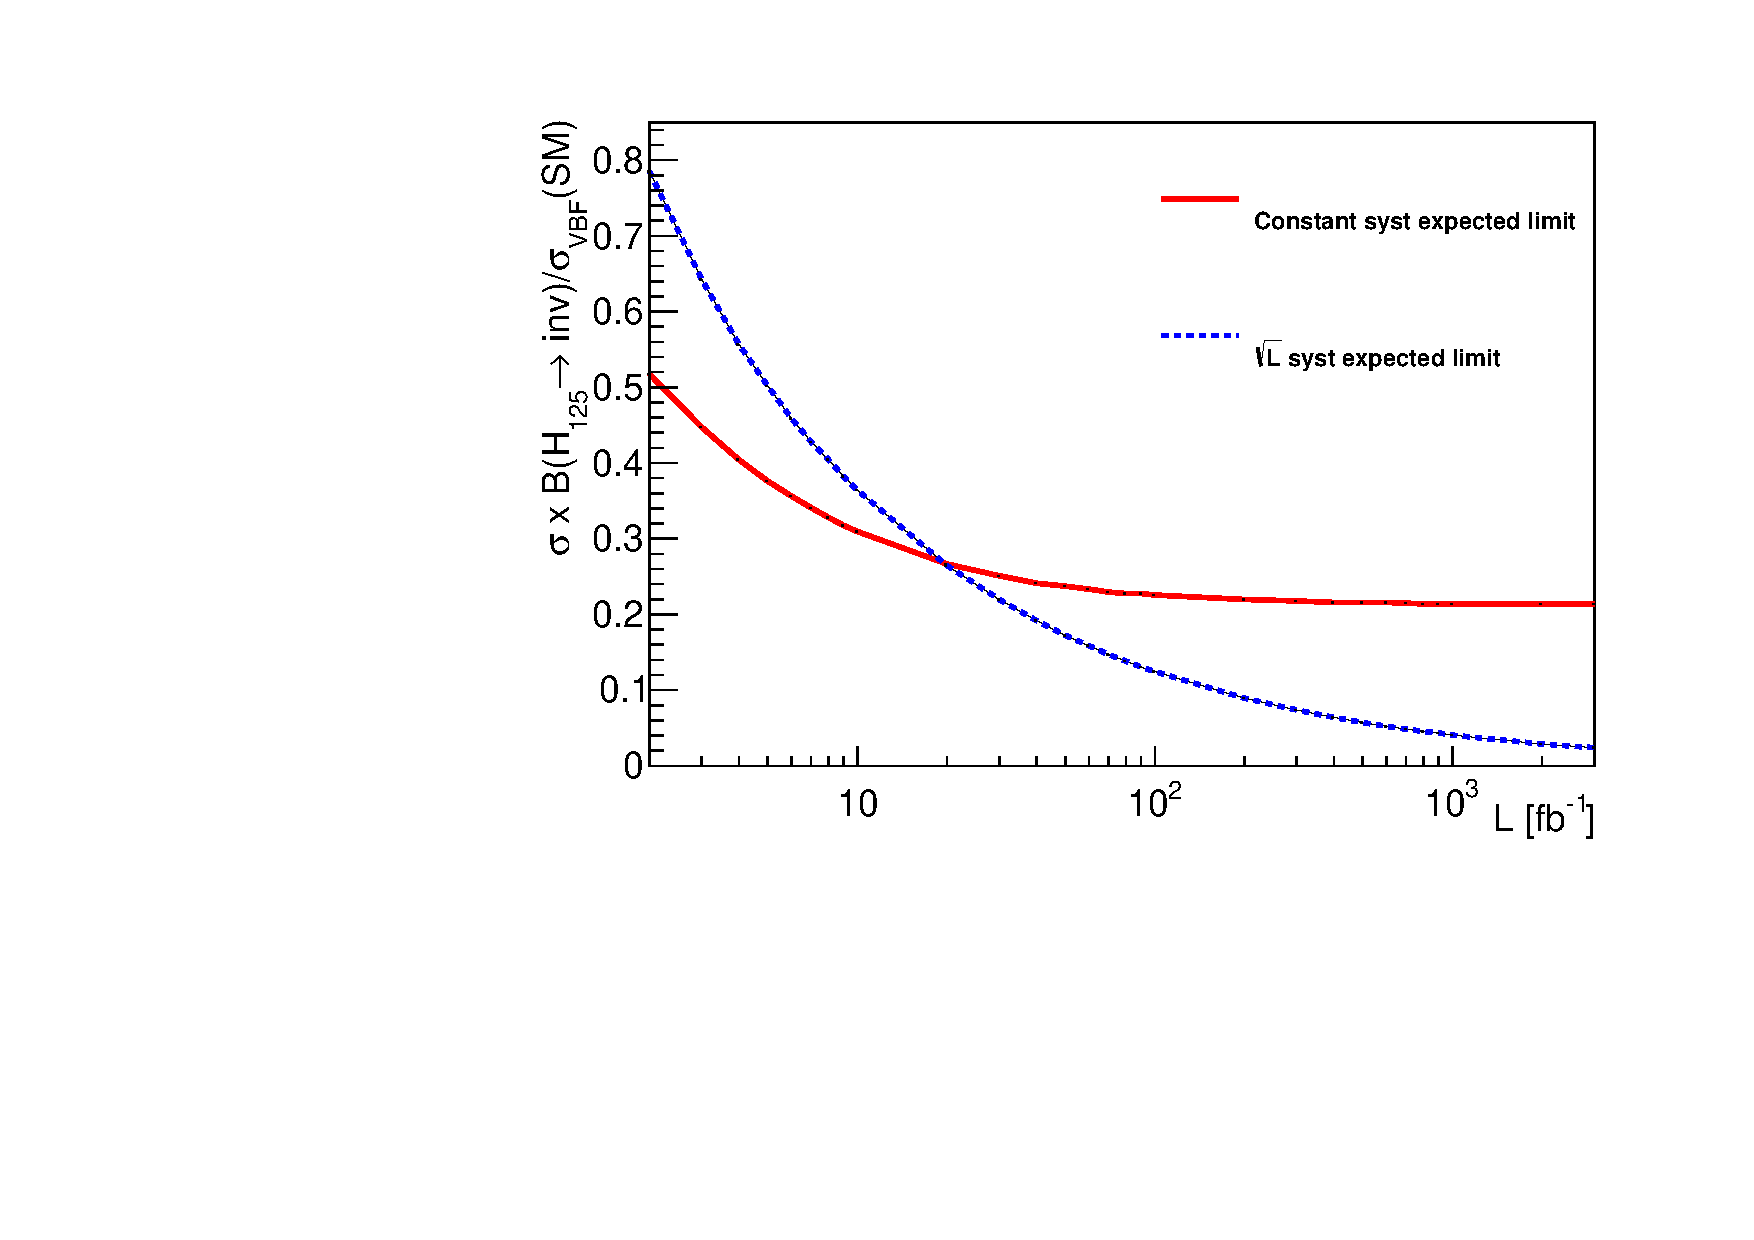
\includegraphics[width=\largefigwidth]{plots/interp/phenoprojectedvbflimit.pdf}}

  \subfloat[]{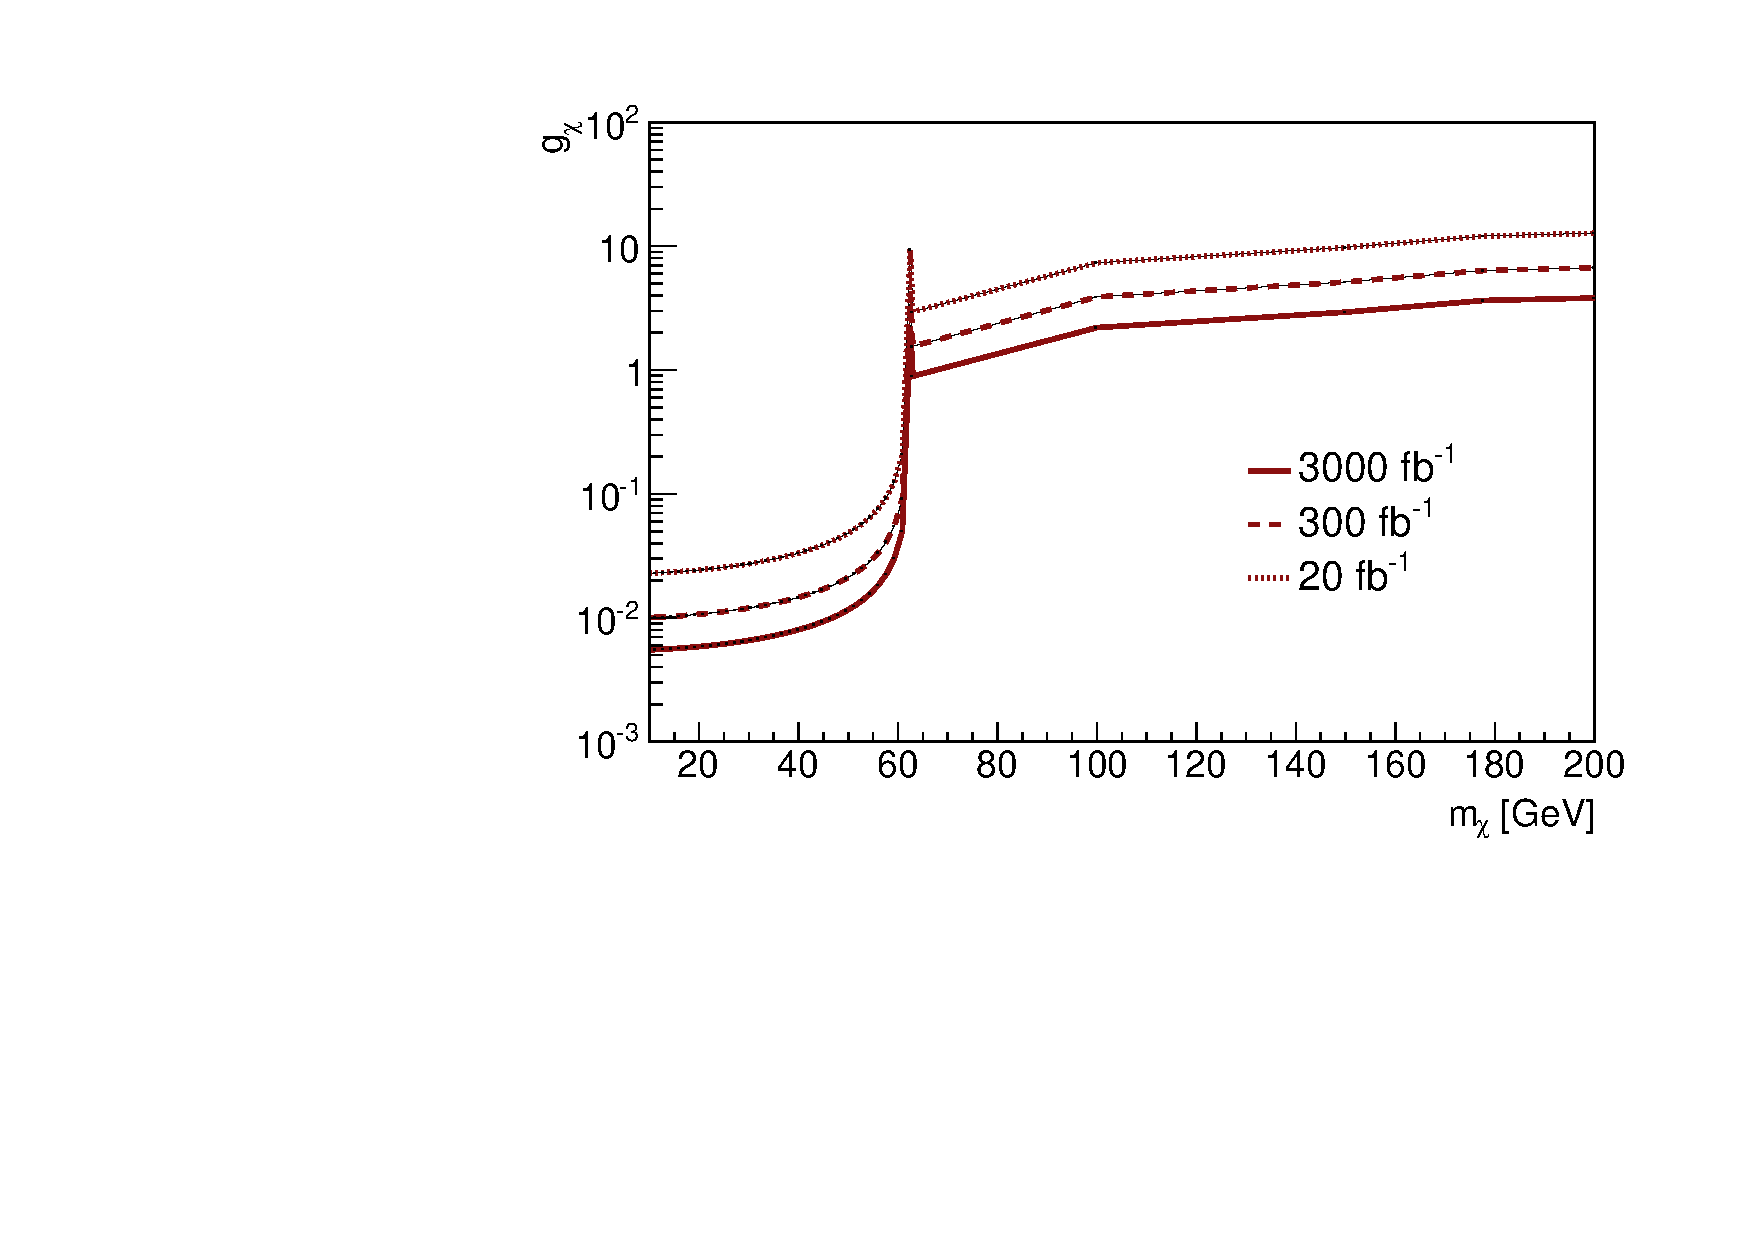
\includegraphics[width=\largefigwidth]{plots/interp/125higgsgchilimit.pdf}}
  \caption{}%??
  \label{fig:smprojectedlimits}
\end{figure}

\begin{figure}
  \subfloat[]{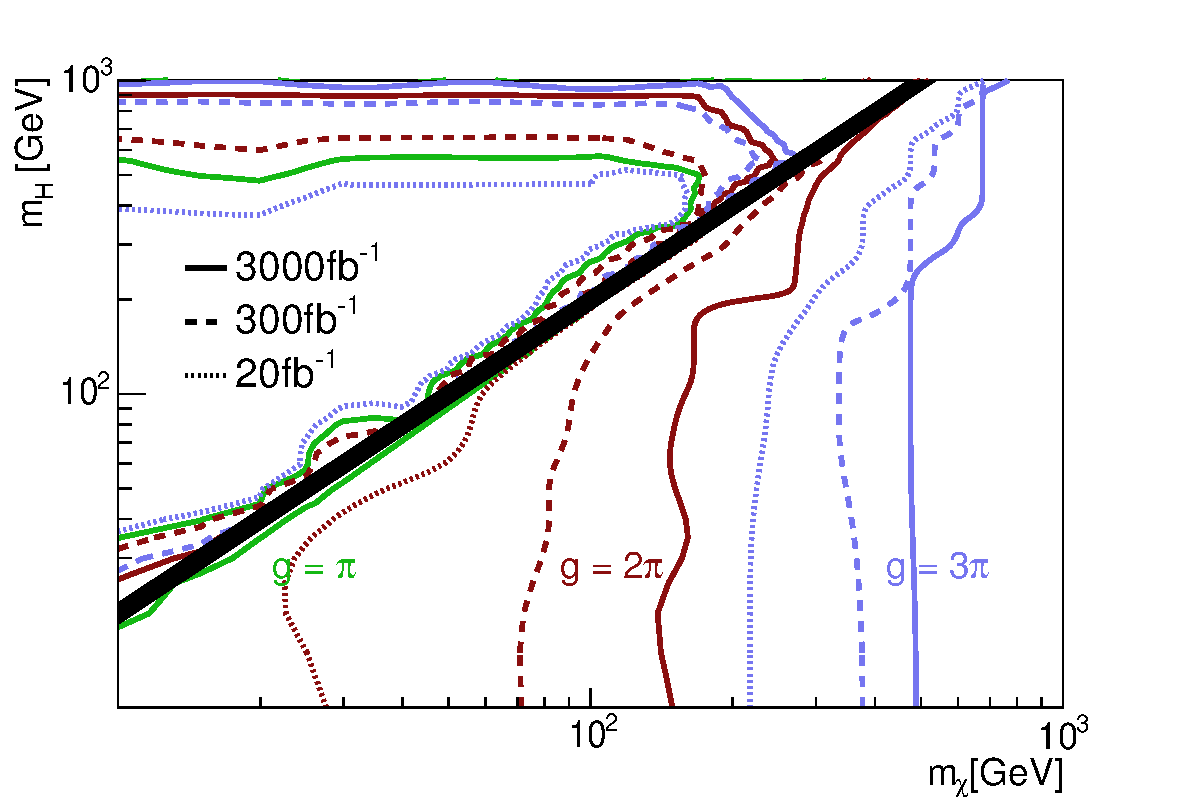
\includegraphics[width=\largefigwidth]{plots/interp/Hplane.pdf}}

  \subfloat[]{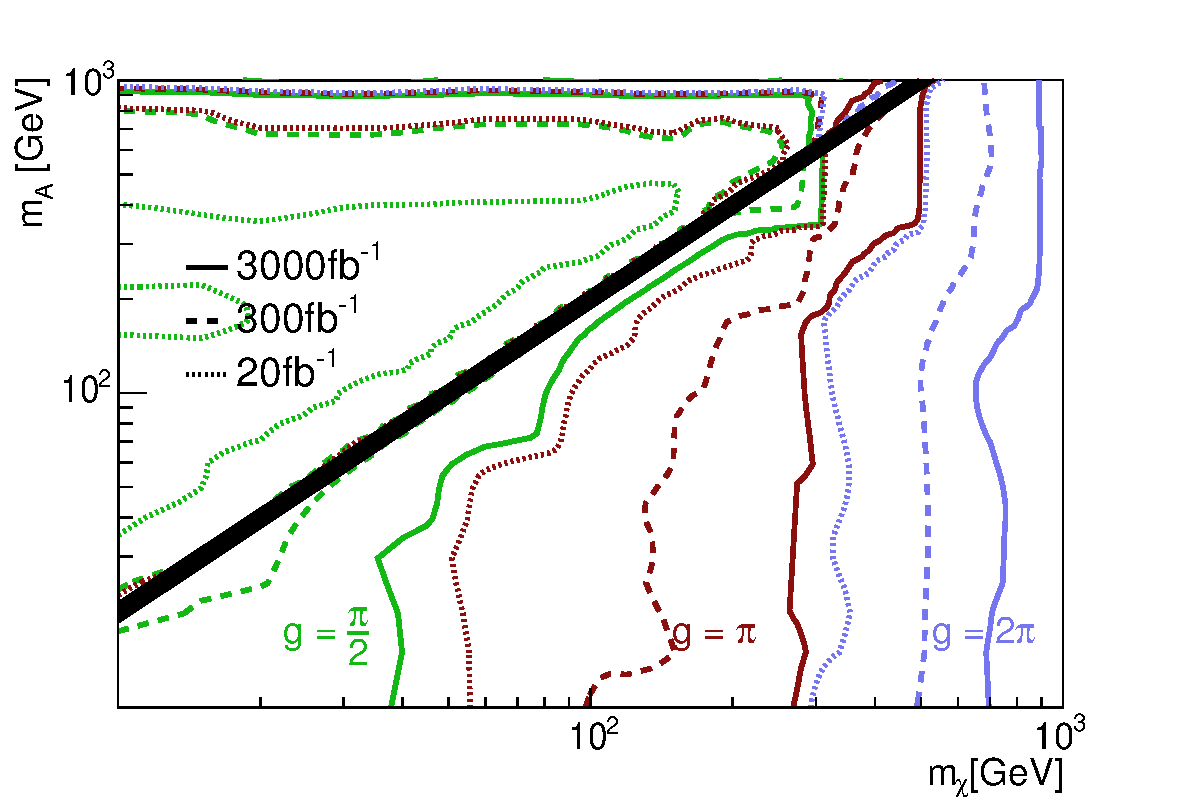
\includegraphics[width=\largefigwidth]{plots/interp/Aplane.pdf}}
  \caption{}%??
  \label{fig:simplifiedmodellimits}
\end{figure}

\begin{figure}
  \subfloat[]{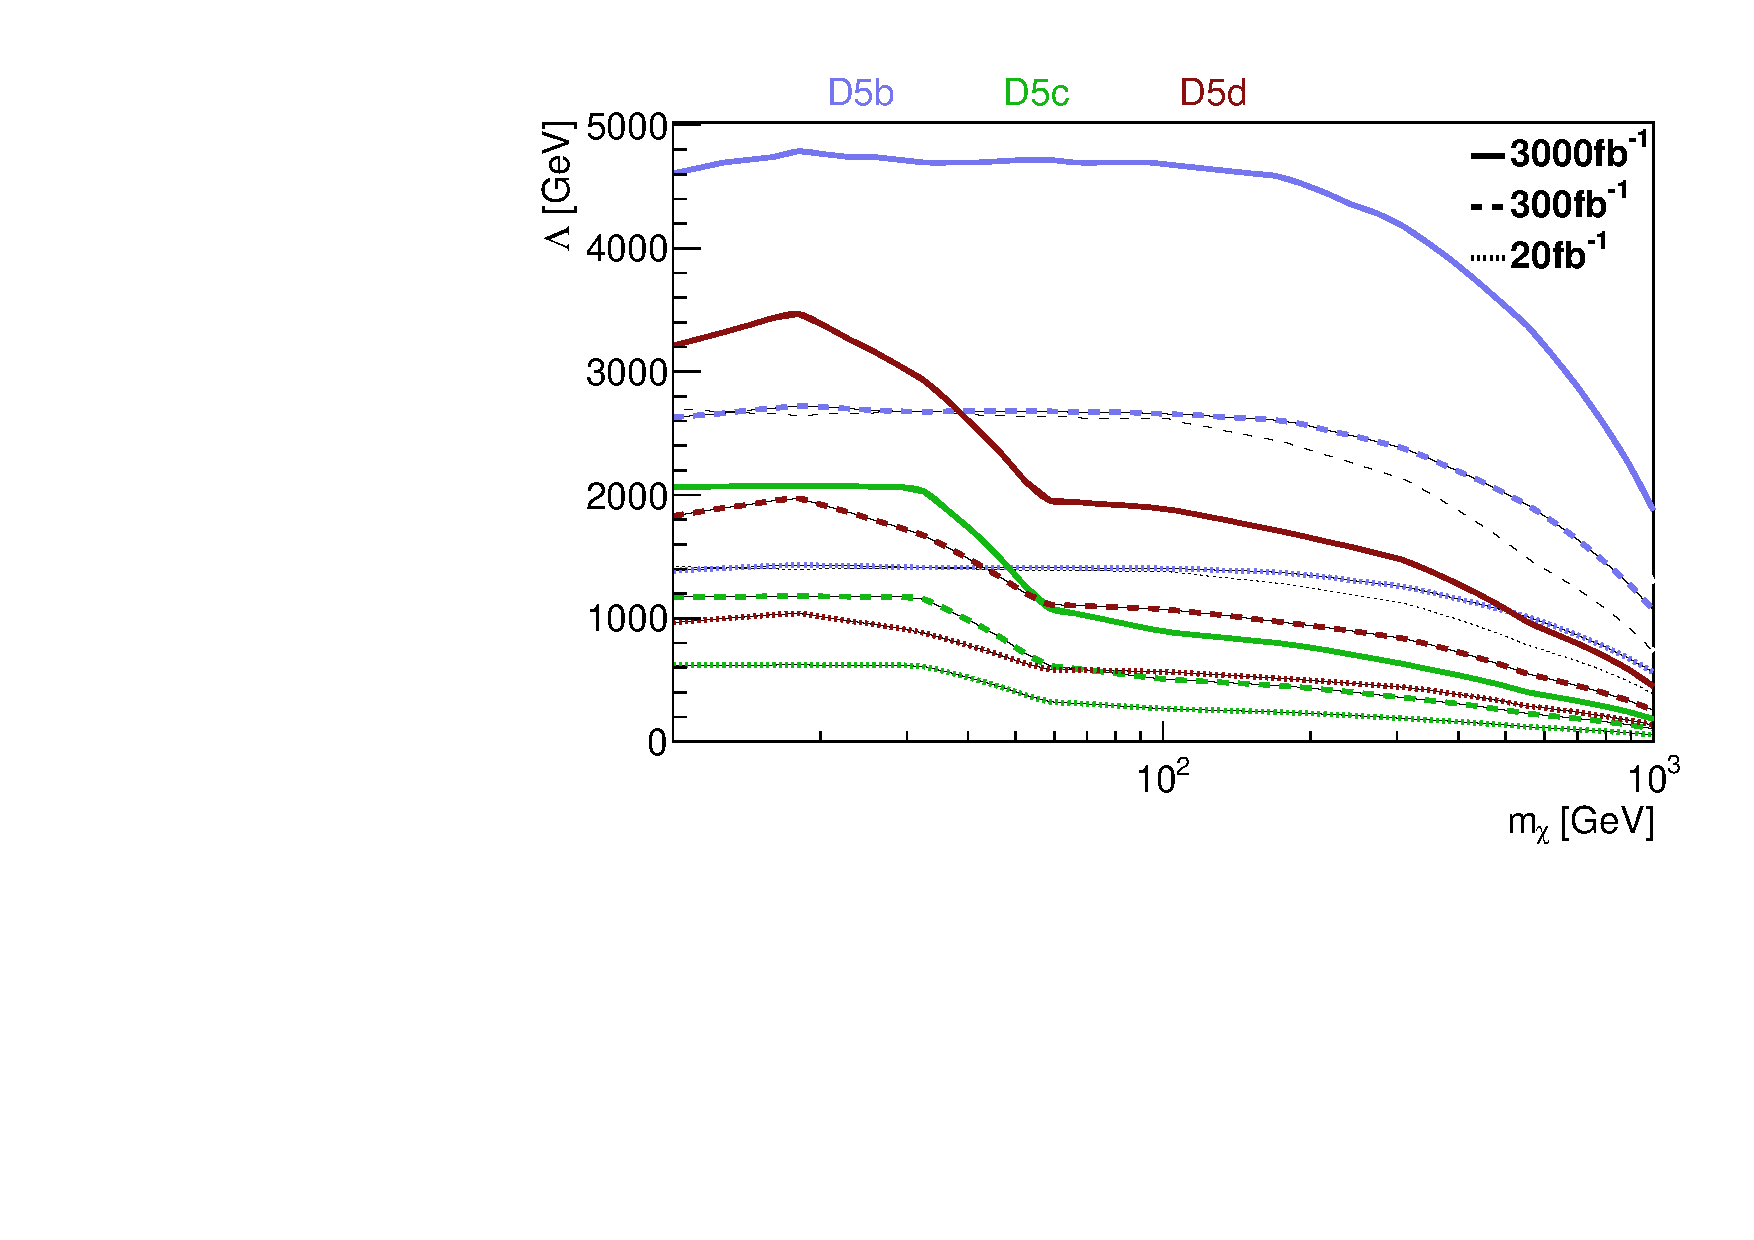
\includegraphics[width=.8\largefigwidth]{plots/interp/D5_multilumi.pdf}}

  \subfloat[]{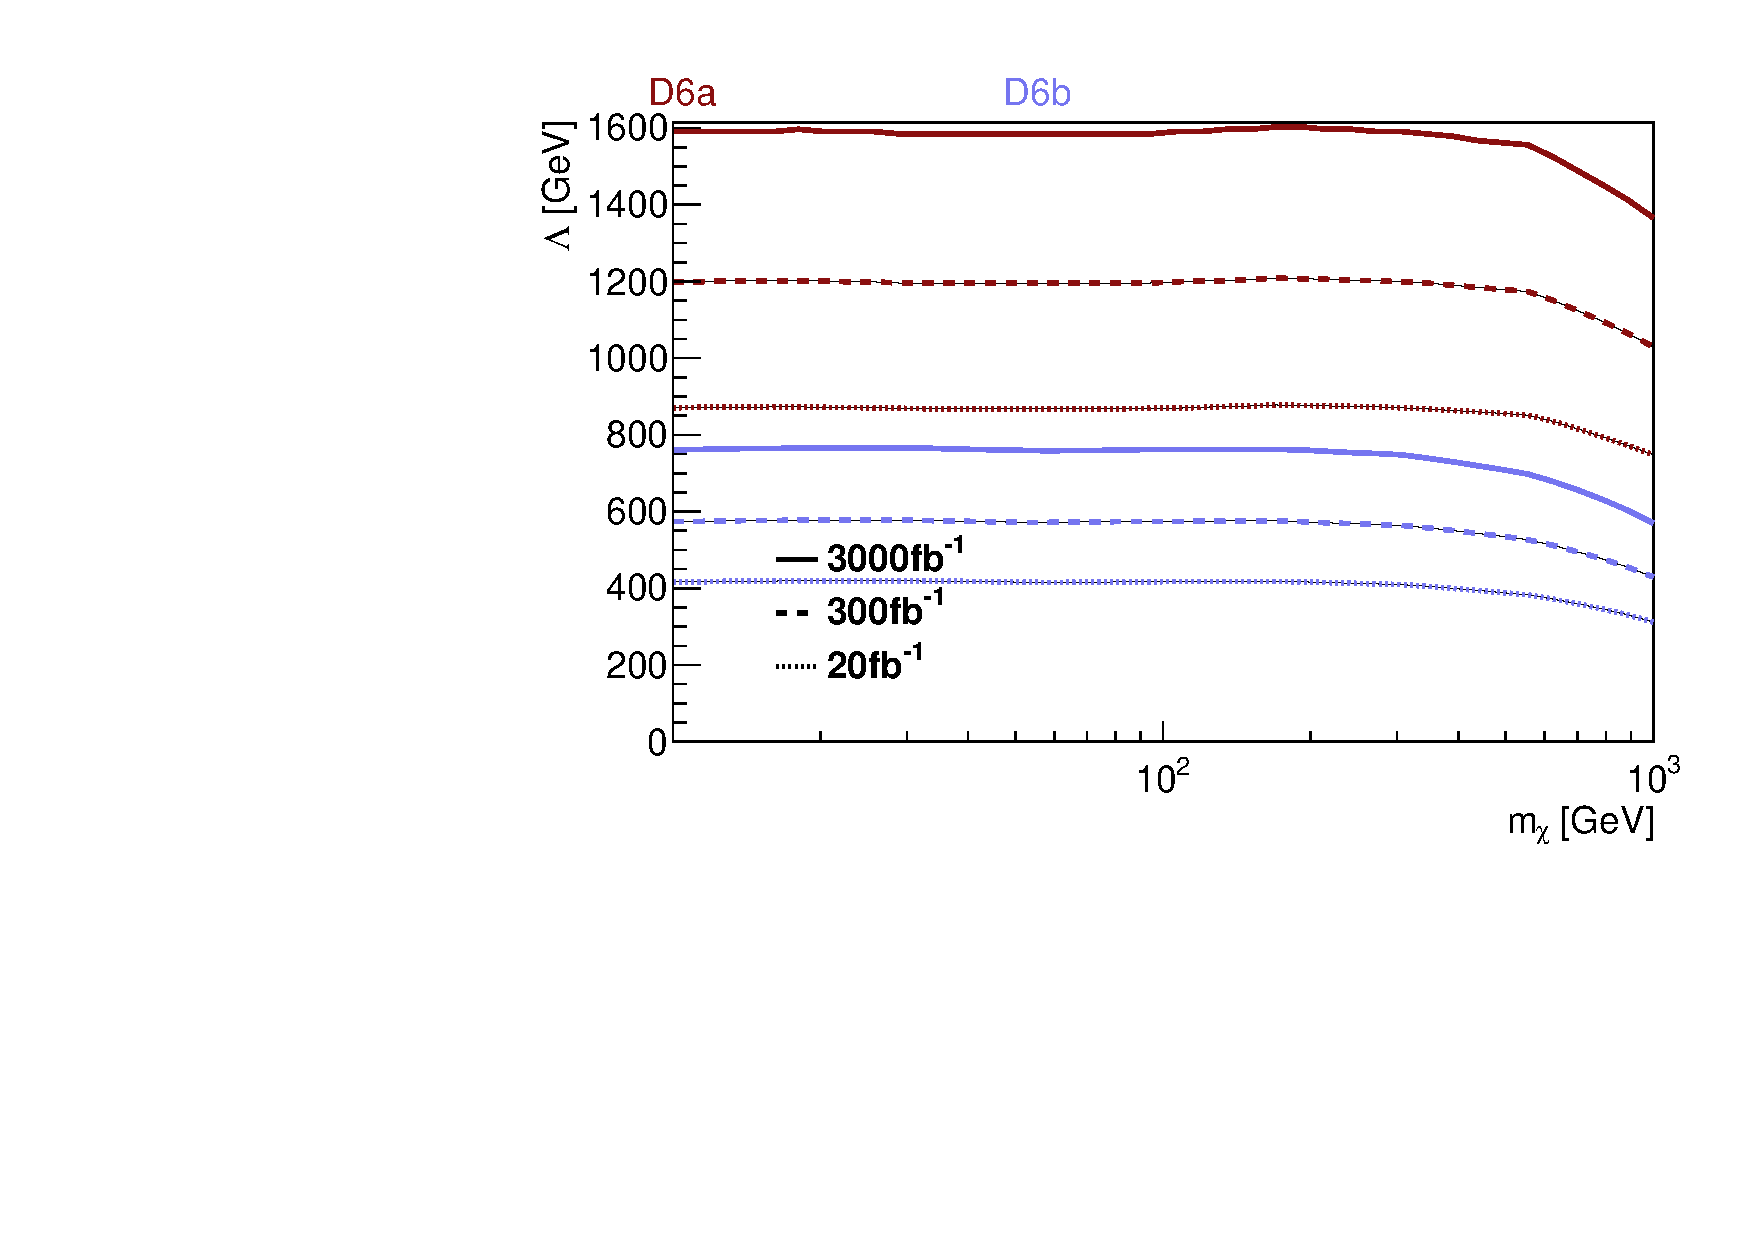
\includegraphics[width=.8\largefigwidth]{plots/interp/D6_2models.pdf}}

  \subfloat[]{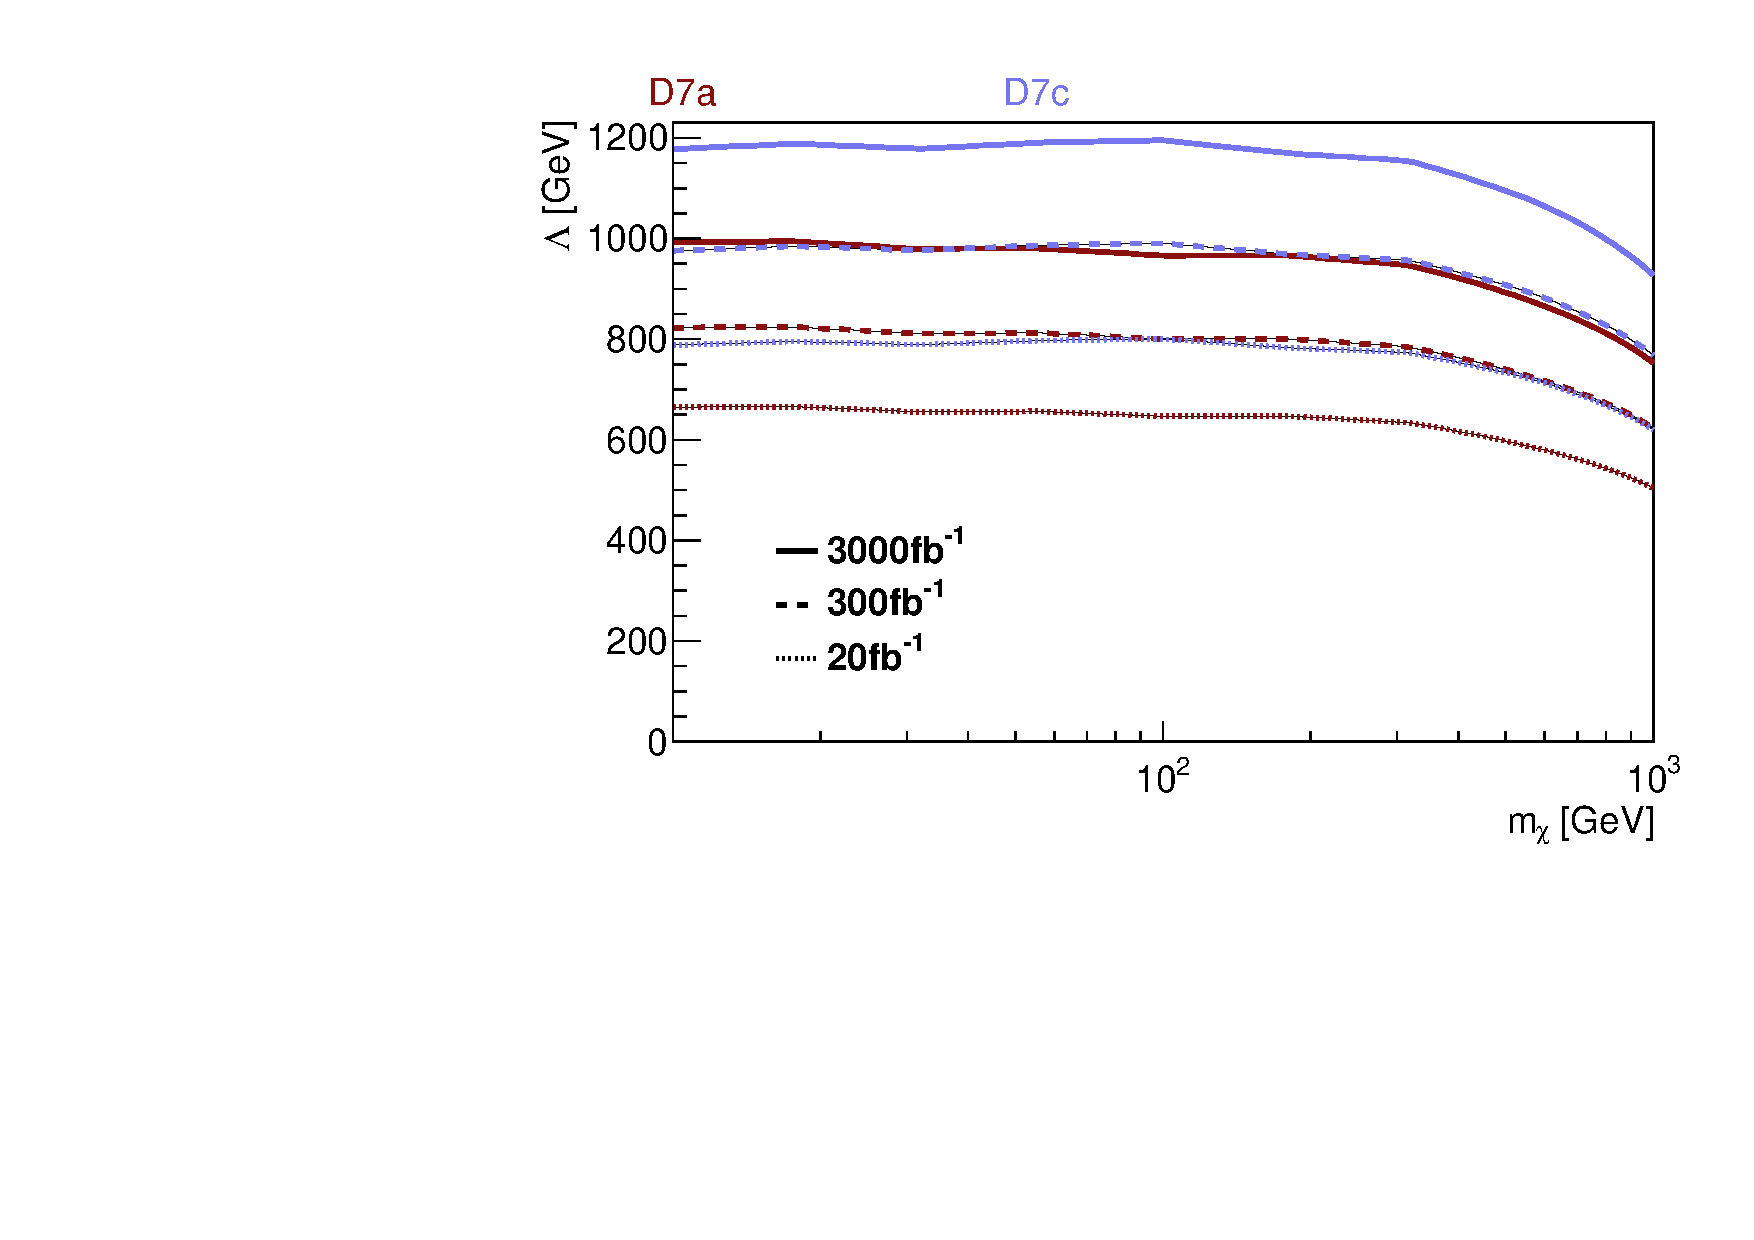
\includegraphics[width=.8\largefigwidth]{plots/interp/D7_2models.pdf}}
  \caption{}%??
  \label{fig:eftlimits}
\end{figure}
